\section{MDD}
Model Driven Development bezeichnet das entwickeln von einem System basierend auf einem Modell, aus dem häufig auch Code generiert werden kann.
Als erstes wird die Systemgerenze festgelegt. Dies soll helfen, die Schnittstellen zur Aussenwelt zu definieren und eine Abgrenzung vom bestehenden zu erhalten. Eine (schlechte) Möglichkeit ist es, das Use Case Diagram zu (miss-)brauchen:
\begin{center}
	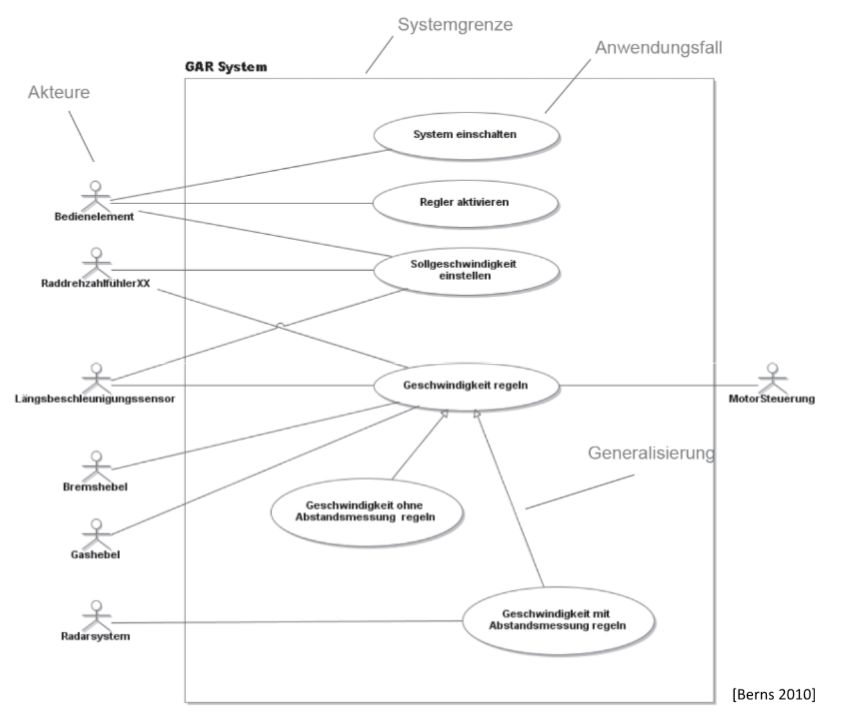
\includegraphics[width=\columnwidth]{Images/use-case}
\end{center}

\subsection{Deployment Diagram}
Bei Embedded Systemen, kommen oft mehrere MCU vor, mittels einem Deployment Diagram kann festgelegt werden, welche Artefakte wo und wie ausgeführt werden. Dabei sind Knoten der Geografischen Orte zu verwenden und die physikalischen Verbinundgen als Linien darzustellen.
\begin{center}
	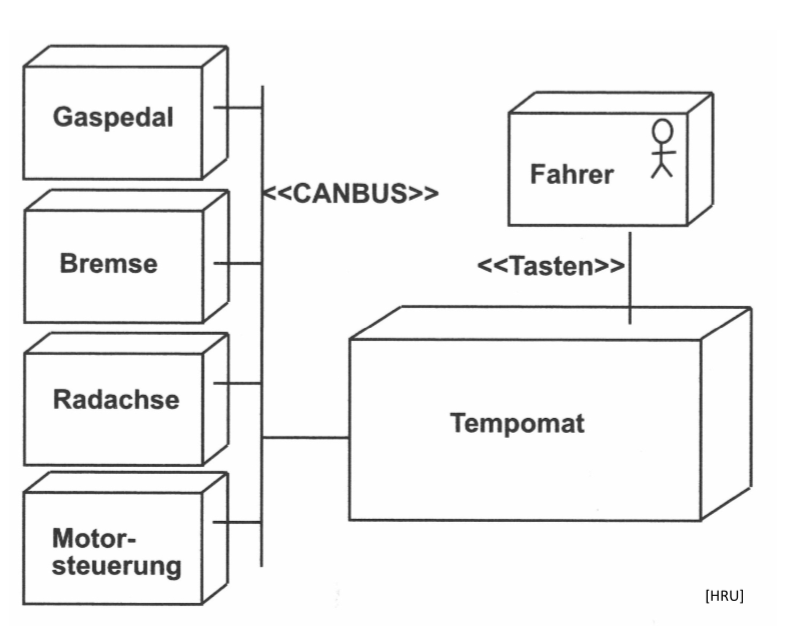
\includegraphics[width=\columnwidth]{Images/deployment-diagram}
\end{center}

\subsection{Sequenz Diagram}
Das Sequenz Diagram eignet sich insbesonders für das Austauschen von Objekten innerhalb einer beschränkten Zeitdauer. 
\begin{center}
	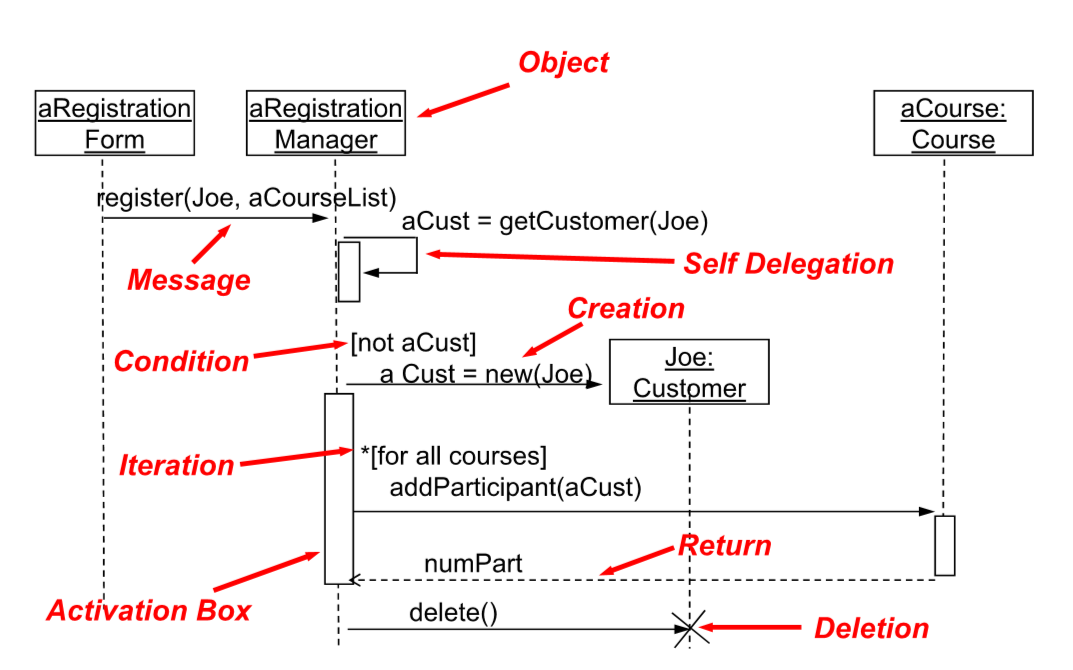
\includegraphics[width=\columnwidth]{Images/seq-diagram}
\end{center}

\subsection{Kommunikations Diagram}
Zeigt die selben Informationen wie Sequenzdiagram an. Der Schwerpunkt liegt aber nicht auf dem Zeitlichen Ablauf, sondern auf dem Informationsfluss zwischen den Objekten.
\begin{center}
	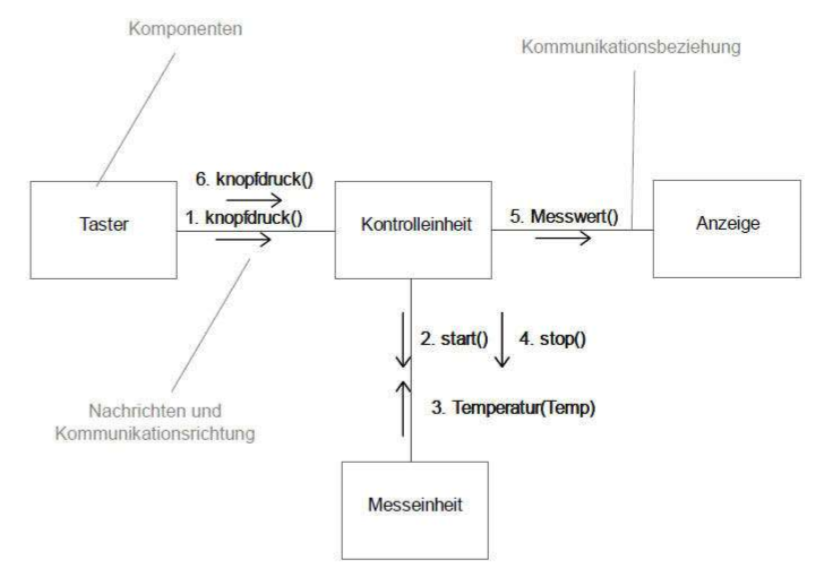
\includegraphics[width=\columnwidth]{Images/kommunikations-diagram}
\end{center}

\subsection{Aktivitäts-Diagram}
Eignet sich für den Sequentiellen Ablauf und weniger für komplexe logische Bedinungen.
\begin{center}
	\includegraphics[width=\columnwidth]{Images/aktivitäts-diagram}
\end{center}
